\section{Decomposition 2: OtherFunctionality (M1, P2, UC11)}

\subsection{Module to decompose}
    In this run we decompose OtherFunctionality.


\subsection{Selected architectural drivers}
    The non-functional drivers for this decomposition are:
    \begin{itemize}
    	\item \emph{M1}: Integrate new sensor or actuator manufacturer
        \item \emph{P2}: Requests to the pluggable data database
    \end{itemize}

    \noindent The related functional drivers are:
    \begin{itemize}
        \item \emph{UC11}: Send pluggable device data (P2) \\
              This use case stores pluggable device data in the pluggable device data storage.
              This could be a sensor reading, or an actuator status.
    \end{itemize}

    \paragraph{Rationale}
    We choose M1 because it belogs to the quality attributes with hight priority. M1 is about
    integration of new sensor or actuator. And it is very important to easily add new devices, because market grows very fast
    and new applications are developing. So we want to focus on this quality attribute
    in the early stages and then based on that create other functionality and components.
    And we also choose P2 because it is related to M1. M1 required minimal changes to data processing and storage,
    so we have to deal with good solution for this topic.  
        
     %Why we do dis???? One was high priority and P2 is related. THey are family and family belongs together.


\subsection{Architectural design}
    % Tactics:
    %     Limit event response? reply within response measure deadlines
    %     Prioritize events
    %     Introduce concurrency
    %     Schedule resources

    \paragraph{Handling new types of pluggable devices for M1}
        The developers have to make changes to: component1, component2, datatype X.
        The new type of sensor needs to be able to be initialised so that it can send data.
        Thus, the PluggableDeviceFacade code that initialises devices should be updated for
        each new type of sensor. The PluggableDeviceData datatype should be updated to
        represent the new type of data. In this case, the new type will have to be added
        to the database that contains all different types of sensor data.

    \paragraph{Data conversions for M1}
        \texttt{The PluggableDeviceDataConverter} is resposible for converting data 
         in system, for instance converting temperature in degrees Fahrenheit 
         to degrees Celsius. System has to work with relevant data, 
         otherwise problem may arise. 
         

    \paragraph{Usage of new data by applications for M1}
        This is possible through the RequestData interface provided by PluggableDeviceDataScheduler.
        The application manager can get device data from the PluggableDeviceDB and return this
        data to applications in the PluggableDeviceData datatype. This datatype can easily be
        updated for new types of pluggable devices.

    \paragraph{Configuration of new device by infrastructure owners for M1}
        Initialisation: IO triggers the initialise() function which has been
        updated for the new pluggable device -> OK\\
        Configure access rights: has absolutely fucking nothing to do with the
        new sensor type -> OK \\
        Consult and configure topology: same as configure access rights

    \paragraph{Scheduling for P2}
        dynamic priority scheduling \\
        tactics: schedule resource, prioritize events, also limit event response?\\
        starvation avoidance

    \paragraph{Pluggable data separation for P2}
        "pluggable data has no impact on other data"
        two databases

    \subsubsection{Alternatives considered}
        \paragraph{Alternatives for solution}
            A discussion of the alternative solutions and why that were not selected.


\subsection{Instantiation and allocation of functionality}
    \paragraph{Decomposition}
        Main aspects of the resulting decomposition.

        \begin{figure}[!htp]
        	\centering
            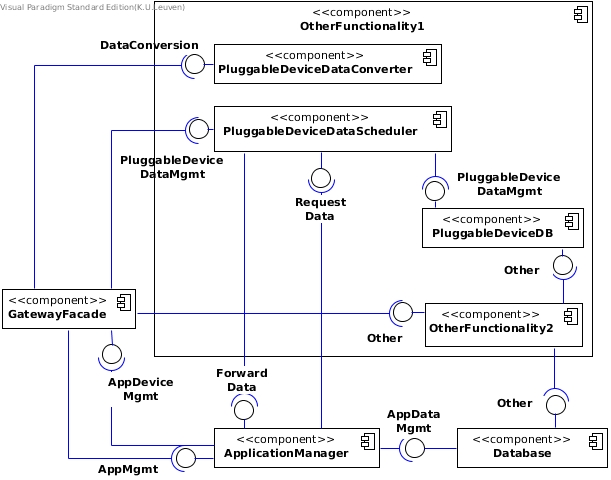
\includegraphics[width=1.00\textwidth]{component-diagram-2}
        	\caption{Component-and-connector diagram of this decomposition.}
            \label{fig:it1-cc_main}
        \end{figure}

    \subparagraph{PluggableDeviceDB}
        store data related to pluggable devices

    \subparagraph{PluggableDeviceDataScheduler}
        scheduling, detect overload mode, store data, forward data

    \subparagraph{PluggableDeviceDataConverter}
        M1: conversion of new type of data of new type of device

    % \paragraph{Behaviour}
        % A SEQUENCE DIAGRAM FOR UC11 WOULD BE ACTUALLY VERY USEFUL (shows how the gateway checks if devices are initialised)
        % REMOVE THIS PART BECAUSE MONEYKA IS LAAAAZZZZYYYYYY BAD STUDENT "IT IS NOT NECESSARY"

    \paragraph{Deployment}
        Rationale of the allocation of components to physical nodes.

        \begin{figure}[!htp]
        	\centering
        	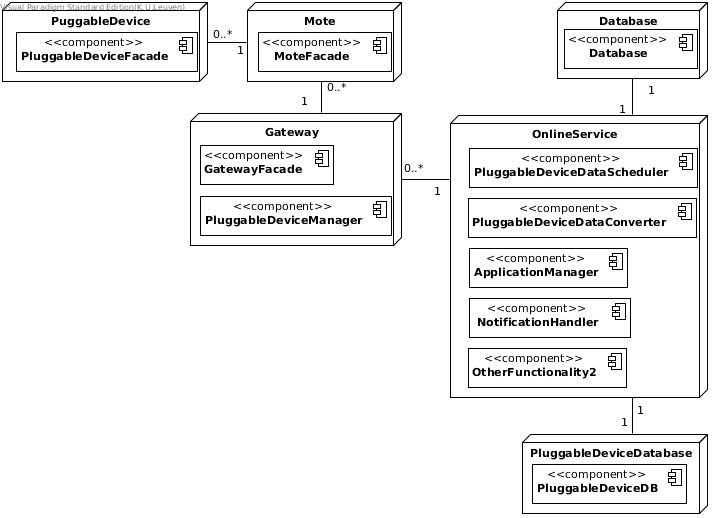
\includegraphics[width=1.00\textwidth]{deployment-diagram-2}
        	\caption{Deployment diagram of this decomposition.
        	}\label{fig:it1-depl_main}
        \end{figure}


\subsection{Interfaces for child modules}

    \subsubsection{GatewayFacade}
        See "\ref{ADD1-int-gatewayfacade}: GatewayFacade" for the rest of the interfaces provided by this component.
        \begin{itemize}
            \item MoteDataMgmt
            \begin{itemize}
                \item \texttt{void sendData(PluggableDeviceData data)}
                \begin{itemize}
                    \item Effect: Sends pluggable device data to the connected mote.
                    \item Exceptions: None
                \end{itemize}
            \end{itemize}

            \item DeviceMgmt
            \begin{itemize}
                \item \texttt{void initialiseDevice(int deviceID, PluggableDeviceSettings settings)}
                \begin{itemize}
                    \item Effect: Initialises a pluggable device for use with the system.
                    \item Exceptions: None
                \end{itemize}
            \end{itemize}

            \item AppDeviceMgmt
            \begin{itemize}
                \item \texttt{void configurePluggableDevice(int deviceID, PluggableDeviceSettings settings)}
                \begin{itemize}
                    \item For: Use case 11 step 3.b
                    \item Effect: Causes certain settings to be set on a pluggable
                          device that the gateway is connected to.
                    \item Exceptions: None
                \end{itemize}
            \end{itemize}
        \end{itemize}

    \subsubsection{MoteFacade}
        See "\ref{add1-int-motefacade}: MoteFacade" for the rest of the interfaces provided by this component.
        \begin{itemize}
            \item PluggableDeviceDataMgmt
            \begin{itemize}
                \item \texttt{void sendData(PluggableDeviceData data)}
                \begin{itemize}
                    \item Effect: Sends pluggable device data to the connected mote.
                    \item Exceptions: None
                \end{itemize}
            \end{itemize}

            \item PluggableDeviceMgmt
            \begin{itemize}
                \item \texttt{void initialise(int deviceID, PluggableDeviceSettings settings)}
                \begin{itemize}
                    \item Effect: Initialises a connected pluggable device according to some settings
                    \item Exceptions: None
                \end{itemize}
            \end{itemize}
        \end{itemize}

    \subsubsection{PluggableDeviceFacade}
        \begin{itemize}
        	\item PluggableDeviceMgmt
        	\begin{itemize}
                \item \texttt{void initialise(PluggableDeviceSettings settings)}
                \begin{itemize}
                    \item Effect: Initialises the pluggable device according to some settings
                    \item Exceptions: None
                \end{itemize}
        	\end{itemize}
        \end{itemize}

    \subsubsection{PluggableDeviceManager}
        \begin{itemize}
        	\item DeviceListMgmt
        	\begin{itemize}
        		\item \texttt{bool isDeviceInitialised(int deviceID)}
        		\begin{itemize}
        			\item Effect: Returns true if the device with id "deviceID" has been initialized.
        			\item Exceptions: None
        		\end{itemize}
        	\end{itemize}
        \end{itemize}

    \subsubsection{PluggableDeviceDataScheduler}
        \begin{itemize}
            \item RequestData
            \begin{itemize}
                \item \texttt{List<PluggableDeviceData> requestData(int applicationID, int deviceID, DateTime from, DateTime to)}
                \begin{itemize}
                    \item Effect: Request data from a specific device in a certain time period
                    \item Exceptions: None
                \end{itemize}
            \end{itemize}

            \item PluggableDeviceDataMgmt
            \begin{itemize}
                \item \texttt{void sendData(PluggableDeviceData data)}
                \begin{itemize}
                    \item Effect: Sends pluggable device data to the scheduler to be processed.
                    \item Exceptions: None
                \end{itemize}
            \end{itemize}
        \end{itemize}

    \subsubsection{PluggableDeviceDB}
        \begin{itemize}
            \item PluggableDeviceDataMgmt
            \begin{itemize}
                \item \texttt{void sendData(PluggableDeviceData data)}
                \begin{itemize}
                    \item Effect: Sends pluggable device data to the DB to be stored.
                    \item Exceptions: None
                \end{itemize}
                \item \texttt{List<PluggableDeviceData> getData(int deviceID, DateTime from, DateTime to)}
                \begin{itemize}
                    \item Effect: Returns data from a specific device in a certain time period.
                    \item Exceptions: None
                \end{itemize}
                \item \texttt{List<int> getApplicationsForDevice(int deviceID)}
                \begin{itemize}
                    \item Effect: Returns a list of applications that can use the device with id "deviceID."
                    \item Exceptions: None
                \end{itemize}
            \end{itemize}
        \end{itemize}


\subsection{Data type definitions}
    \paragraph{DateTime} Represents an instant in time, typically expressed as a date and time of day.


\subsection{Verify and refine}
    Completely handled: M1, P2, UC11 \\

    \noindent This section describes per component which (parts of) the remaining
    requirements it is responsible for.

    \paragraph{ApplicationManager}
        \begin{itemize}
            \item  \emph{Av2}: Application failure \\
                   Prevention: a, b \\
                   Detection: a, b, c \\
                   Resolution: a, b, c
           \item \emph{P1}: Large number of users: c
           \item \emph{M2}: Big data analytics on pluggable data and/or application usage data: d, e
           \item \emph{U1}: Application updates: a, b, c, d
           \item \emph{U2}: Easy Installation: e
           \item \emph{U12}: Perform actuation command
           \item \emph{UC17}: Activate an application: 3, 4
        \end{itemize}

    \paragraph{Database}
        \begin{itemize}
          	\item None
        \end{itemize}

    \paragraph{GatewayFacade}
        \begin{itemize}
            \item \emph{Av1}: Communication between SIoTIP gateway and Online Service \\
                               Resolution: b, c, d
            \item \emph{U2}: Easy Installation: a, c, d
        \end{itemize}

    \paragraph{MoteFacade}
        \begin{itemize}
            \item \emph{U2}: Easy Installation: b, c, d
            \item \emph{UC4}: Install mote: 1, 2
            \item \emph{UC5}: Uninstall mote: 1
            \item \emph{UC6}: Insert a pluggable device into a mote: 2
            \item \emph{UC7}: Remove a pluggable device from its mote: 2
        \end{itemize}

    \paragraph{NotificationHandler}
        \begin{itemize}
            \item \emph{UC16}: Consult notification message: 5
            \item \emph{UC17}: Activate an application: 5, 6
        \end{itemize}

    \paragraph{OtherFunctionality}
        \begin{itemize}
            \item \emph{Av1}: Communication between SIoTIP gateway and Online Service \\
                               Detection: a, b, c, d
                               Resolution: a
           	\item \emph{P1}: Large number of users: a
            \item \emph{M2}: Big data analytics on pluggable data and/or application usage data: a
            \item \emph{U2}: Easy Installation: e
            \item \emph{UC1}: Register a customer organisation
            \item \emph{UC2}: Register an end-user
            \item \emph{UC3}: Unregister an end user
            \item \emph{UC4}: Install mote: 3
            \item \emph{UC5}: Uninstall mote: 2.b
            \item \emph{UC6}: Insert a pluggable device into a mote: 3: topology part; alternative 3a.1.b
            \item \emph{UC7}: Remove a pluggable device from its mote: 3.b
            \item \emph{UC8}: Initialise a pluggable device: 1, 2, 4
            \item \emph{UC9}: Configure pluggable device access rights
            \item \emph{UC10}: Consult and configure the topology
            \item \emph{UC13}: Configure pluggable device
            \item \emph{UC16}: Consult notification message: 1, 2, 3, 4
            \item \emph{UC17}: Activate an application: 1, 2
            \item \emph{UC19}: Subscribe to application
            \item \emph{UC20}: Unsubscribe from application
            \item \emph{UC21}: Send invoice
            \item \emph{UC22}: Upload an application
            \item \emph{UC23}: Consult application statistics
            \item \emph{UC24}: Consult historical data
            \item \emph{UC25}: Access topology and available devices
            \item \emph{UC26}: Send application command or message to external front-end
            \item \emph{UC27}: Receive application command or message to external front-end
            \item \emph{UC28}: Log in
            \item \emph{UC29}: Log out
        \end{itemize}

    \paragraph{PluggableDeviceDB}
        \begin{itemize}
            \item \emph{M2}: Big data analytics on pluggable data and/or application usage data: b
        \end{itemize}

    \paragraph{PluggableDeviceFacade}
        \begin{itemize}
        	\item \emph{U2}: Easy Installation: d
        \end{itemize}

    \paragraph{PluggableDeviceManager}
        \begin{itemize}
            \item \emph{U2}: Easy Installation: c, d
            \item \emph{UC4}: Install mote: 4
            \item \emph{UC5}: Uninstall mote: 2
            \item \emph{UC6}: Insert a pluggable device into a mote: 3: uninitialised part; alternative 3a.1 3a.2 3a.4; 4
            \item \emph{UC7}: Remove a pluggable device from its mote: 3.a, 3.c
            \item \emph{UC8}: Initialise a pluggable device: 3,
        \end{itemize}

    \paragraph{PluggableDeviceDataScheduler}
        \begin{itemize}
            \item \emph{P1}: Large number of users: b
            \item \emph{M2}: Big data analytics on pluggable data and/or application usage data: b, c
        \end{itemize}
